% Created by tikzDevice version 0.7.0 on 2014-11-07 12:14:39
% !TEX encoding = UTF-8 Unicode
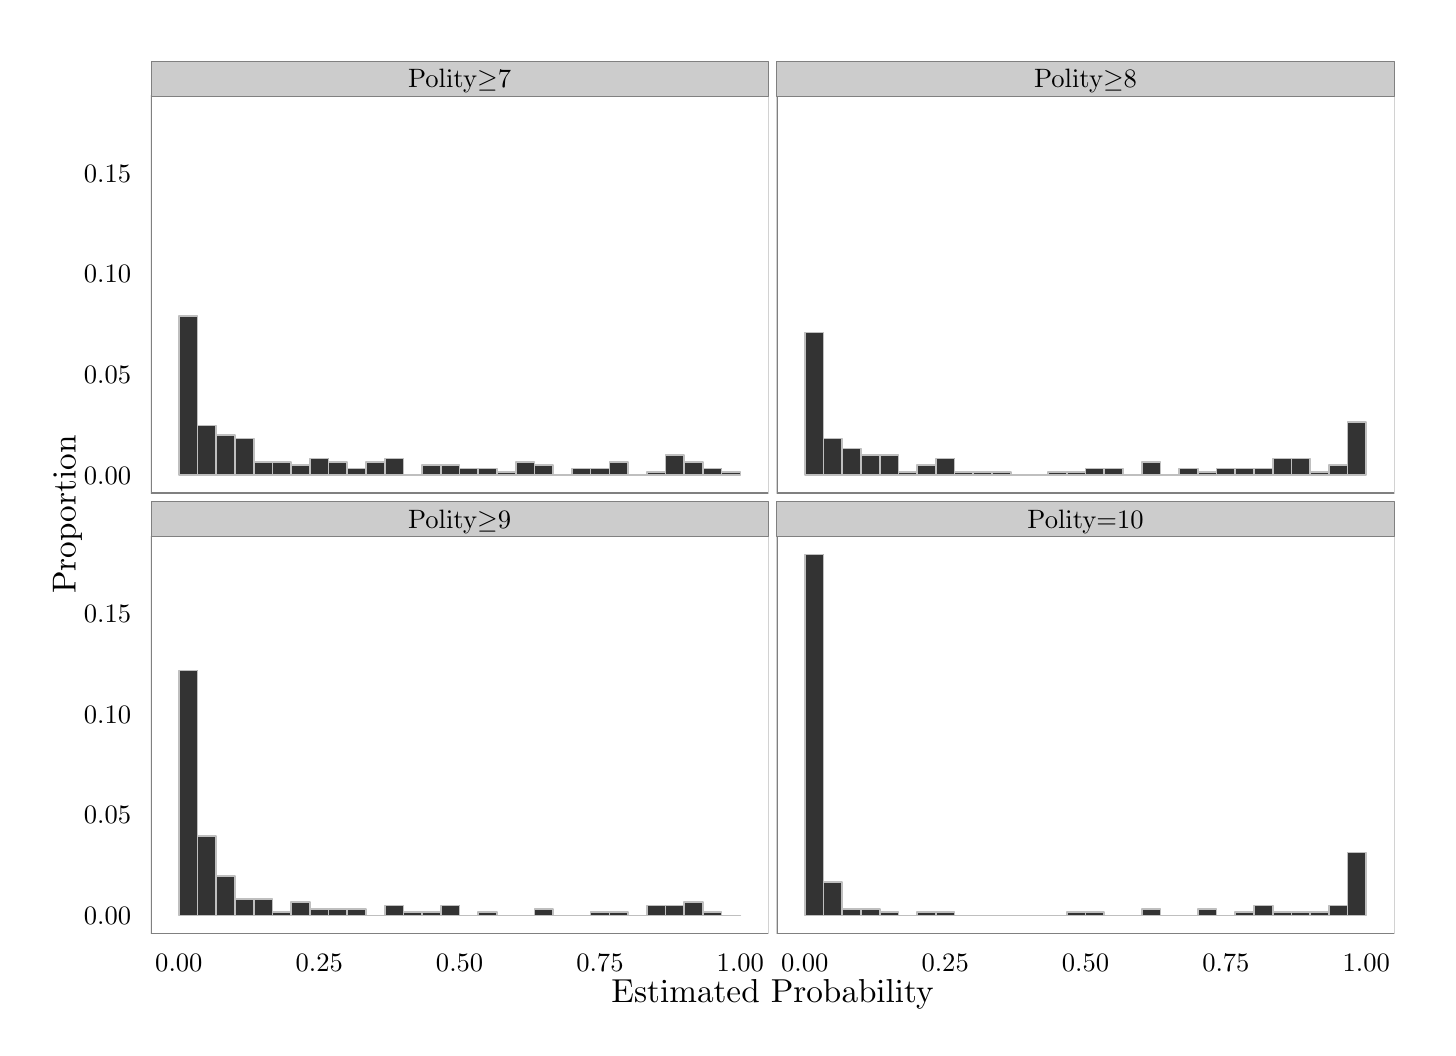
\begin{tikzpicture}[x=1pt,y=1pt]
\definecolor[named]{fillColor}{rgb}{1.00,1.00,1.00}
\path[use as bounding box,fill=fillColor,fill opacity=0.00] (0,0) rectangle (505.89,361.35);
\begin{scope}
\path[clip] (  0.00,  0.00) rectangle (505.89,361.35);
\definecolor[named]{drawColor}{rgb}{1.00,1.00,1.00}
\definecolor[named]{fillColor}{rgb}{1.00,1.00,1.00}

\path[draw=drawColor,line width= 0.6pt,line join=round,line cap=round,fill=fillColor] (  0.00,  0.00) rectangle (505.89,361.35);
\end{scope}
\begin{scope}
\path[clip] ( 44.49,193.18) rectangle (267.66,336.67);
\definecolor[named]{fillColor}{rgb}{1.00,1.00,1.00}

\path[fill=fillColor] ( 44.49,193.18) rectangle (267.66,336.67);
\definecolor[named]{drawColor}{rgb}{0.75,0.75,0.75}
\definecolor[named]{fillColor}{rgb}{0.20,0.20,0.20}

\path[draw=drawColor,line width= 0.6pt,line join=round,fill=fillColor] ( 54.63,199.70) rectangle ( 61.39,257.14);

\path[draw=drawColor,line width= 0.6pt,line join=round,fill=fillColor] ( 61.39,199.70) rectangle ( 68.16,217.65);

\path[draw=drawColor,line width= 0.6pt,line join=round,fill=fillColor] ( 68.16,199.70) rectangle ( 74.92,214.06);

\path[draw=drawColor,line width= 0.6pt,line join=round,fill=fillColor] ( 74.92,199.70) rectangle ( 81.68,212.86);

\path[draw=drawColor,line width= 0.6pt,line join=round,fill=fillColor] ( 81.68,199.70) rectangle ( 88.44,204.49);

\path[draw=drawColor,line width= 0.6pt,line join=round,fill=fillColor] ( 88.44,199.70) rectangle ( 95.21,204.49);

\path[draw=drawColor,line width= 0.6pt,line join=round,fill=fillColor] ( 95.21,199.70) rectangle (101.97,203.29);

\path[draw=drawColor,line width= 0.6pt,line join=round,fill=fillColor] (101.97,199.70) rectangle (108.73,205.68);

\path[draw=drawColor,line width= 0.6pt,line join=round,fill=fillColor] (108.73,199.70) rectangle (115.50,204.49);

\path[draw=drawColor,line width= 0.6pt,line join=round,fill=fillColor] (115.50,199.70) rectangle (122.26,202.09);

\path[draw=drawColor,line width= 0.6pt,line join=round,fill=fillColor] (122.26,199.70) rectangle (129.02,204.49);

\path[draw=drawColor,line width= 0.6pt,line join=round,fill=fillColor] (129.02,199.70) rectangle (135.78,205.68);

\path[draw=drawColor,line width= 0.6pt,line join=round,fill=fillColor] (135.78,199.70) rectangle (142.55,199.70);

\path[draw=drawColor,line width= 0.6pt,line join=round,fill=fillColor] (142.55,199.70) rectangle (149.31,203.29);

\path[draw=drawColor,line width= 0.6pt,line join=round,fill=fillColor] (149.31,199.70) rectangle (156.07,203.29);

\path[draw=drawColor,line width= 0.6pt,line join=round,fill=fillColor] (156.07,199.70) rectangle (162.84,202.09);

\path[draw=drawColor,line width= 0.6pt,line join=round,fill=fillColor] (162.84,199.70) rectangle (169.60,202.09);

\path[draw=drawColor,line width= 0.6pt,line join=round,fill=fillColor] (169.60,199.70) rectangle (176.36,200.89);

\path[draw=drawColor,line width= 0.6pt,line join=round,fill=fillColor] (176.36,199.70) rectangle (183.12,204.49);

\path[draw=drawColor,line width= 0.6pt,line join=round,fill=fillColor] (183.12,199.70) rectangle (189.89,203.29);

\path[draw=drawColor,line width= 0.6pt,line join=round,fill=fillColor] (189.89,199.70) rectangle (196.65,199.70);

\path[draw=drawColor,line width= 0.6pt,line join=round,fill=fillColor] (196.65,199.70) rectangle (203.41,202.09);

\path[draw=drawColor,line width= 0.6pt,line join=round,fill=fillColor] (203.41,199.70) rectangle (210.18,202.09);

\path[draw=drawColor,line width= 0.6pt,line join=round,fill=fillColor] (210.18,199.70) rectangle (216.94,204.49);

\path[draw=drawColor,line width= 0.6pt,line join=round,fill=fillColor] (216.94,199.70) rectangle (223.70,199.70);

\path[draw=drawColor,line width= 0.6pt,line join=round,fill=fillColor] (223.70,199.70) rectangle (230.46,200.89);

\path[draw=drawColor,line width= 0.6pt,line join=round,fill=fillColor] (230.46,199.70) rectangle (237.23,206.88);

\path[draw=drawColor,line width= 0.6pt,line join=round,fill=fillColor] (237.23,199.70) rectangle (243.99,204.49);

\path[draw=drawColor,line width= 0.6pt,line join=round,fill=fillColor] (243.99,199.70) rectangle (250.75,202.09);

\path[draw=drawColor,line width= 0.6pt,line join=round,fill=fillColor] (250.75,199.70) rectangle (257.52,200.89);
\definecolor[named]{drawColor}{rgb}{0.50,0.50,0.50}

\path[draw=drawColor,line width= 0.6pt,line join=round,line cap=round] ( 44.49,193.18) rectangle (267.66,336.67);
\end{scope}
\begin{scope}
\path[clip] (270.67,193.18) rectangle (493.85,336.67);
\definecolor[named]{fillColor}{rgb}{1.00,1.00,1.00}

\path[fill=fillColor] (270.67,193.18) rectangle (493.85,336.67);
\definecolor[named]{drawColor}{rgb}{0.75,0.75,0.75}
\definecolor[named]{fillColor}{rgb}{0.20,0.20,0.20}

\path[draw=drawColor,line width= 0.6pt,line join=round,fill=fillColor] (280.82,199.70) rectangle (287.58,251.16);

\path[draw=drawColor,line width= 0.6pt,line join=round,fill=fillColor] (287.58,199.70) rectangle (294.34,212.86);

\path[draw=drawColor,line width= 0.6pt,line join=round,fill=fillColor] (294.34,199.70) rectangle (301.10,209.27);

\path[draw=drawColor,line width= 0.6pt,line join=round,fill=fillColor] (301.10,199.70) rectangle (307.87,206.88);

\path[draw=drawColor,line width= 0.6pt,line join=round,fill=fillColor] (307.87,199.70) rectangle (314.63,206.88);

\path[draw=drawColor,line width= 0.6pt,line join=round,fill=fillColor] (314.63,199.70) rectangle (321.39,200.89);

\path[draw=drawColor,line width= 0.6pt,line join=round,fill=fillColor] (321.39,199.70) rectangle (328.16,203.29);

\path[draw=drawColor,line width= 0.6pt,line join=round,fill=fillColor] (328.16,199.70) rectangle (334.92,205.68);

\path[draw=drawColor,line width= 0.6pt,line join=round,fill=fillColor] (334.92,199.70) rectangle (341.68,200.89);

\path[draw=drawColor,line width= 0.6pt,line join=round,fill=fillColor] (341.68,199.70) rectangle (348.44,200.89);

\path[draw=drawColor,line width= 0.6pt,line join=round,fill=fillColor] (348.44,199.70) rectangle (355.21,200.89);

\path[draw=drawColor,line width= 0.6pt,line join=round,fill=fillColor] (355.21,199.70) rectangle (361.97,199.70);

\path[draw=drawColor,line width= 0.6pt,line join=round,fill=fillColor] (361.97,199.70) rectangle (368.73,199.70);

\path[draw=drawColor,line width= 0.6pt,line join=round,fill=fillColor] (368.73,199.70) rectangle (375.50,200.89);

\path[draw=drawColor,line width= 0.6pt,line join=round,fill=fillColor] (375.50,199.70) rectangle (382.26,200.89);

\path[draw=drawColor,line width= 0.6pt,line join=round,fill=fillColor] (382.26,199.70) rectangle (389.02,202.09);

\path[draw=drawColor,line width= 0.6pt,line join=round,fill=fillColor] (389.02,199.70) rectangle (395.78,202.09);

\path[draw=drawColor,line width= 0.6pt,line join=round,fill=fillColor] (395.78,199.70) rectangle (402.55,199.70);

\path[draw=drawColor,line width= 0.6pt,line join=round,fill=fillColor] (402.55,199.70) rectangle (409.31,204.49);

\path[draw=drawColor,line width= 0.6pt,line join=round,fill=fillColor] (409.31,199.70) rectangle (416.07,199.70);

\path[draw=drawColor,line width= 0.6pt,line join=round,fill=fillColor] (416.07,199.70) rectangle (422.84,202.09);

\path[draw=drawColor,line width= 0.6pt,line join=round,fill=fillColor] (422.84,199.70) rectangle (429.60,200.89);

\path[draw=drawColor,line width= 0.6pt,line join=round,fill=fillColor] (429.60,199.70) rectangle (436.36,202.09);

\path[draw=drawColor,line width= 0.6pt,line join=round,fill=fillColor] (436.36,199.70) rectangle (443.12,202.09);

\path[draw=drawColor,line width= 0.6pt,line join=round,fill=fillColor] (443.12,199.70) rectangle (449.89,202.09);

\path[draw=drawColor,line width= 0.6pt,line join=round,fill=fillColor] (449.89,199.70) rectangle (456.65,205.68);

\path[draw=drawColor,line width= 0.6pt,line join=round,fill=fillColor] (456.65,199.70) rectangle (463.41,205.68);

\path[draw=drawColor,line width= 0.6pt,line join=round,fill=fillColor] (463.41,199.70) rectangle (470.18,200.89);

\path[draw=drawColor,line width= 0.6pt,line join=round,fill=fillColor] (470.18,199.70) rectangle (476.94,203.29);

\path[draw=drawColor,line width= 0.6pt,line join=round,fill=fillColor] (476.94,199.70) rectangle (483.70,218.85);
\definecolor[named]{drawColor}{rgb}{0.50,0.50,0.50}

\path[draw=drawColor,line width= 0.6pt,line join=round,line cap=round] (270.67,193.18) rectangle (493.85,336.67);
\end{scope}
\begin{scope}
\path[clip] ( 44.49, 34.03) rectangle (267.66,177.53);
\definecolor[named]{fillColor}{rgb}{1.00,1.00,1.00}

\path[fill=fillColor] ( 44.49, 34.03) rectangle (267.66,177.53);
\definecolor[named]{drawColor}{rgb}{0.75,0.75,0.75}
\definecolor[named]{fillColor}{rgb}{0.20,0.20,0.20}

\path[draw=drawColor,line width= 0.6pt,line join=round,fill=fillColor] ( 54.63, 40.56) rectangle ( 61.39,129.12);

\path[draw=drawColor,line width= 0.6pt,line join=round,fill=fillColor] ( 61.39, 40.56) rectangle ( 68.16, 69.28);

\path[draw=drawColor,line width= 0.6pt,line join=round,fill=fillColor] ( 68.16, 40.56) rectangle ( 74.92, 54.92);

\path[draw=drawColor,line width= 0.6pt,line join=round,fill=fillColor] ( 74.92, 40.56) rectangle ( 81.68, 46.54);

\path[draw=drawColor,line width= 0.6pt,line join=round,fill=fillColor] ( 81.68, 40.56) rectangle ( 88.44, 46.54);

\path[draw=drawColor,line width= 0.6pt,line join=round,fill=fillColor] ( 88.44, 40.56) rectangle ( 95.21, 41.75);

\path[draw=drawColor,line width= 0.6pt,line join=round,fill=fillColor] ( 95.21, 40.56) rectangle (101.97, 45.34);

\path[draw=drawColor,line width= 0.6pt,line join=round,fill=fillColor] (101.97, 40.56) rectangle (108.73, 42.95);

\path[draw=drawColor,line width= 0.6pt,line join=round,fill=fillColor] (108.73, 40.56) rectangle (115.50, 42.95);

\path[draw=drawColor,line width= 0.6pt,line join=round,fill=fillColor] (115.50, 40.56) rectangle (122.26, 42.95);

\path[draw=drawColor,line width= 0.6pt,line join=round,fill=fillColor] (122.26, 40.56) rectangle (129.02, 40.56);

\path[draw=drawColor,line width= 0.6pt,line join=round,fill=fillColor] (129.02, 40.56) rectangle (135.78, 44.15);

\path[draw=drawColor,line width= 0.6pt,line join=round,fill=fillColor] (135.78, 40.56) rectangle (142.55, 41.75);

\path[draw=drawColor,line width= 0.6pt,line join=round,fill=fillColor] (142.55, 40.56) rectangle (149.31, 41.75);

\path[draw=drawColor,line width= 0.6pt,line join=round,fill=fillColor] (149.31, 40.56) rectangle (156.07, 44.15);

\path[draw=drawColor,line width= 0.6pt,line join=round,fill=fillColor] (156.07, 40.56) rectangle (162.84, 40.56);

\path[draw=drawColor,line width= 0.6pt,line join=round,fill=fillColor] (162.84, 40.56) rectangle (169.60, 41.75);

\path[draw=drawColor,line width= 0.6pt,line join=round,fill=fillColor] (169.60, 40.56) rectangle (176.36, 40.56);

\path[draw=drawColor,line width= 0.6pt,line join=round,fill=fillColor] (176.36, 40.56) rectangle (183.12, 40.56);

\path[draw=drawColor,line width= 0.6pt,line join=round,fill=fillColor] (183.12, 40.56) rectangle (189.89, 42.95);

\path[draw=drawColor,line width= 0.6pt,line join=round,fill=fillColor] (189.89, 40.56) rectangle (196.65, 40.56);

\path[draw=drawColor,line width= 0.6pt,line join=round,fill=fillColor] (196.65, 40.56) rectangle (203.41, 40.56);

\path[draw=drawColor,line width= 0.6pt,line join=round,fill=fillColor] (203.41, 40.56) rectangle (210.18, 41.75);

\path[draw=drawColor,line width= 0.6pt,line join=round,fill=fillColor] (210.18, 40.56) rectangle (216.94, 41.75);

\path[draw=drawColor,line width= 0.6pt,line join=round,fill=fillColor] (216.94, 40.56) rectangle (223.70, 40.56);

\path[draw=drawColor,line width= 0.6pt,line join=round,fill=fillColor] (223.70, 40.56) rectangle (230.46, 44.15);

\path[draw=drawColor,line width= 0.6pt,line join=round,fill=fillColor] (230.46, 40.56) rectangle (237.23, 44.15);

\path[draw=drawColor,line width= 0.6pt,line join=round,fill=fillColor] (237.23, 40.56) rectangle (243.99, 45.34);

\path[draw=drawColor,line width= 0.6pt,line join=round,fill=fillColor] (243.99, 40.56) rectangle (250.75, 41.75);

\path[draw=drawColor,line width= 0.6pt,line join=round,fill=fillColor] (250.75, 40.56) rectangle (257.52, 40.56);
\definecolor[named]{drawColor}{rgb}{0.50,0.50,0.50}

\path[draw=drawColor,line width= 0.6pt,line join=round,line cap=round] ( 44.49, 34.03) rectangle (267.66,177.53);
\end{scope}
\begin{scope}
\path[clip] (270.67, 34.03) rectangle (493.85,177.53);
\definecolor[named]{fillColor}{rgb}{1.00,1.00,1.00}

\path[fill=fillColor] (270.67, 34.03) rectangle (493.85,177.53);
\definecolor[named]{drawColor}{rgb}{0.75,0.75,0.75}
\definecolor[named]{fillColor}{rgb}{0.20,0.20,0.20}

\path[draw=drawColor,line width= 0.6pt,line join=round,fill=fillColor] (280.82, 40.56) rectangle (287.58,171.01);

\path[draw=drawColor,line width= 0.6pt,line join=round,fill=fillColor] (287.58, 40.56) rectangle (294.34, 52.53);

\path[draw=drawColor,line width= 0.6pt,line join=round,fill=fillColor] (294.34, 40.56) rectangle (301.10, 42.95);

\path[draw=drawColor,line width= 0.6pt,line join=round,fill=fillColor] (301.10, 40.56) rectangle (307.87, 42.95);

\path[draw=drawColor,line width= 0.6pt,line join=round,fill=fillColor] (307.87, 40.56) rectangle (314.63, 41.75);

\path[draw=drawColor,line width= 0.6pt,line join=round,fill=fillColor] (314.63, 40.56) rectangle (321.39, 40.56);

\path[draw=drawColor,line width= 0.6pt,line join=round,fill=fillColor] (321.39, 40.56) rectangle (328.16, 41.75);

\path[draw=drawColor,line width= 0.6pt,line join=round,fill=fillColor] (328.16, 40.56) rectangle (334.92, 41.75);

\path[draw=drawColor,line width= 0.6pt,line join=round,fill=fillColor] (334.92, 40.56) rectangle (341.68, 40.56);

\path[draw=drawColor,line width= 0.6pt,line join=round,fill=fillColor] (341.68, 40.56) rectangle (348.44, 40.56);

\path[draw=drawColor,line width= 0.6pt,line join=round,fill=fillColor] (348.44, 40.56) rectangle (355.21, 40.56);

\path[draw=drawColor,line width= 0.6pt,line join=round,fill=fillColor] (355.21, 40.56) rectangle (361.97, 40.56);

\path[draw=drawColor,line width= 0.6pt,line join=round,fill=fillColor] (361.97, 40.56) rectangle (368.73, 40.56);

\path[draw=drawColor,line width= 0.6pt,line join=round,fill=fillColor] (368.73, 40.56) rectangle (375.50, 40.56);

\path[draw=drawColor,line width= 0.6pt,line join=round,fill=fillColor] (375.50, 40.56) rectangle (382.26, 41.75);

\path[draw=drawColor,line width= 0.6pt,line join=round,fill=fillColor] (382.26, 40.56) rectangle (389.02, 41.75);

\path[draw=drawColor,line width= 0.6pt,line join=round,fill=fillColor] (389.02, 40.56) rectangle (395.78, 40.56);

\path[draw=drawColor,line width= 0.6pt,line join=round,fill=fillColor] (395.78, 40.56) rectangle (402.55, 40.56);

\path[draw=drawColor,line width= 0.6pt,line join=round,fill=fillColor] (402.55, 40.56) rectangle (409.31, 42.95);

\path[draw=drawColor,line width= 0.6pt,line join=round,fill=fillColor] (409.31, 40.56) rectangle (416.07, 40.56);

\path[draw=drawColor,line width= 0.6pt,line join=round,fill=fillColor] (416.07, 40.56) rectangle (422.84, 40.56);

\path[draw=drawColor,line width= 0.6pt,line join=round,fill=fillColor] (422.84, 40.56) rectangle (429.60, 42.95);

\path[draw=drawColor,line width= 0.6pt,line join=round,fill=fillColor] (429.60, 40.56) rectangle (436.36, 40.56);

\path[draw=drawColor,line width= 0.6pt,line join=round,fill=fillColor] (436.36, 40.56) rectangle (443.12, 41.75);

\path[draw=drawColor,line width= 0.6pt,line join=round,fill=fillColor] (443.12, 40.56) rectangle (449.89, 44.15);

\path[draw=drawColor,line width= 0.6pt,line join=round,fill=fillColor] (449.89, 40.56) rectangle (456.65, 41.75);

\path[draw=drawColor,line width= 0.6pt,line join=round,fill=fillColor] (456.65, 40.56) rectangle (463.41, 41.75);

\path[draw=drawColor,line width= 0.6pt,line join=round,fill=fillColor] (463.41, 40.56) rectangle (470.18, 41.75);

\path[draw=drawColor,line width= 0.6pt,line join=round,fill=fillColor] (470.18, 40.56) rectangle (476.94, 44.15);

\path[draw=drawColor,line width= 0.6pt,line join=round,fill=fillColor] (476.94, 40.56) rectangle (483.70, 63.30);
\definecolor[named]{drawColor}{rgb}{0.50,0.50,0.50}

\path[draw=drawColor,line width= 0.6pt,line join=round,line cap=round] (270.67, 34.03) rectangle (493.85,177.53);
\end{scope}
\begin{scope}
\path[clip] (  0.00,  0.00) rectangle (505.89,361.35);
\definecolor[named]{drawColor}{rgb}{0.50,0.50,0.50}
\definecolor[named]{fillColor}{rgb}{0.80,0.80,0.80}

\path[draw=drawColor,line width= 0.2pt,line join=round,line cap=round,fill=fillColor] ( 44.49,336.67) rectangle (267.66,349.31);
\definecolor[named]{drawColor}{rgb}{0.00,0.00,0.00}

\node[text=drawColor,anchor=base,inner sep=0pt, outer sep=0pt, scale=  0.96] at (156.07,339.68) {Polity$\geq$7};
\end{scope}
\begin{scope}
\path[clip] (  0.00,  0.00) rectangle (505.89,361.35);
\definecolor[named]{drawColor}{rgb}{0.50,0.50,0.50}
\definecolor[named]{fillColor}{rgb}{0.80,0.80,0.80}

\path[draw=drawColor,line width= 0.2pt,line join=round,line cap=round,fill=fillColor] (270.67,336.67) rectangle (493.85,349.31);
\definecolor[named]{drawColor}{rgb}{0.00,0.00,0.00}

\node[text=drawColor,anchor=base,inner sep=0pt, outer sep=0pt, scale=  0.96] at (382.26,339.68) {Polity$\geq$8};
\end{scope}
\begin{scope}
\path[clip] (  0.00,  0.00) rectangle (505.89,361.35);
\definecolor[named]{drawColor}{rgb}{0.50,0.50,0.50}
\definecolor[named]{fillColor}{rgb}{0.80,0.80,0.80}

\path[draw=drawColor,line width= 0.2pt,line join=round,line cap=round,fill=fillColor] ( 44.49,177.53) rectangle (267.66,190.16);
\definecolor[named]{drawColor}{rgb}{0.00,0.00,0.00}

\node[text=drawColor,anchor=base,inner sep=0pt, outer sep=0pt, scale=  0.96] at (156.07,180.54) {Polity$\geq$9};
\end{scope}
\begin{scope}
\path[clip] (  0.00,  0.00) rectangle (505.89,361.35);
\definecolor[named]{drawColor}{rgb}{0.50,0.50,0.50}
\definecolor[named]{fillColor}{rgb}{0.80,0.80,0.80}

\path[draw=drawColor,line width= 0.2pt,line join=round,line cap=round,fill=fillColor] (270.67,177.53) rectangle (493.85,190.16);
\definecolor[named]{drawColor}{rgb}{0.00,0.00,0.00}

\node[text=drawColor,anchor=base,inner sep=0pt, outer sep=0pt, scale=  0.96] at (382.26,180.54) {Polity$=$10};
\end{scope}
\begin{scope}
\path[clip] (  0.00,  0.00) rectangle (505.89,361.35);
\definecolor[named]{drawColor}{rgb}{0.00,0.00,0.00}

\node[text=drawColor,anchor=base east,inner sep=0pt, outer sep=0pt, scale=  0.96] at ( 37.37,196.39) {0.00};

\node[text=drawColor,anchor=base east,inner sep=0pt, outer sep=0pt, scale=  0.96] at ( 37.37,232.77) {0.05};

\node[text=drawColor,anchor=base east,inner sep=0pt, outer sep=0pt, scale=  0.96] at ( 37.37,269.16) {0.10};

\node[text=drawColor,anchor=base east,inner sep=0pt, outer sep=0pt, scale=  0.96] at ( 37.37,305.54) {0.15};
\end{scope}
\begin{scope}
\path[clip] (  0.00,  0.00) rectangle (505.89,361.35);
\definecolor[named]{drawColor}{rgb}{0.00,0.00,0.00}

\node[text=drawColor,anchor=base east,inner sep=0pt, outer sep=0pt, scale=  0.96] at ( 37.37, 37.25) {0.00};

\node[text=drawColor,anchor=base east,inner sep=0pt, outer sep=0pt, scale=  0.96] at ( 37.37, 73.63) {0.05};

\node[text=drawColor,anchor=base east,inner sep=0pt, outer sep=0pt, scale=  0.96] at ( 37.37,110.02) {0.10};

\node[text=drawColor,anchor=base east,inner sep=0pt, outer sep=0pt, scale=  0.96] at ( 37.37,146.40) {0.15};
\end{scope}
\begin{scope}
\path[clip] (  0.00,  0.00) rectangle (505.89,361.35);
\definecolor[named]{drawColor}{rgb}{0.00,0.00,0.00}

\node[text=drawColor,anchor=base,inner sep=0pt, outer sep=0pt, scale=  0.96] at ( 54.63, 20.31) {0.00};

\node[text=drawColor,anchor=base,inner sep=0pt, outer sep=0pt, scale=  0.96] at (105.35, 20.31) {0.25};

\node[text=drawColor,anchor=base,inner sep=0pt, outer sep=0pt, scale=  0.96] at (156.07, 20.31) {0.50};

\node[text=drawColor,anchor=base,inner sep=0pt, outer sep=0pt, scale=  0.96] at (206.79, 20.31) {0.75};

\node[text=drawColor,anchor=base,inner sep=0pt, outer sep=0pt, scale=  0.96] at (257.52, 20.31) {1.00};
\end{scope}
\begin{scope}
\path[clip] (  0.00,  0.00) rectangle (505.89,361.35);
\definecolor[named]{drawColor}{rgb}{0.00,0.00,0.00}

\node[text=drawColor,anchor=base,inner sep=0pt, outer sep=0pt, scale=  0.96] at (280.82, 20.31) {0.00};

\node[text=drawColor,anchor=base,inner sep=0pt, outer sep=0pt, scale=  0.96] at (331.54, 20.31) {0.25};

\node[text=drawColor,anchor=base,inner sep=0pt, outer sep=0pt, scale=  0.96] at (382.26, 20.31) {0.50};

\node[text=drawColor,anchor=base,inner sep=0pt, outer sep=0pt, scale=  0.96] at (432.98, 20.31) {0.75};

\node[text=drawColor,anchor=base,inner sep=0pt, outer sep=0pt, scale=  0.96] at (483.70, 20.31) {1.00};
\end{scope}
\begin{scope}
\path[clip] (  0.00,  0.00) rectangle (505.89,361.35);
\definecolor[named]{drawColor}{rgb}{0.00,0.00,0.00}

\node[text=drawColor,anchor=base,inner sep=0pt, outer sep=0pt, scale=  1.20] at (269.17,  9.03) {Estimated Probability};
\end{scope}
\begin{scope}
\path[clip] (  0.00,  0.00) rectangle (505.89,361.35);
\definecolor[named]{drawColor}{rgb}{0.00,0.00,0.00}

\node[text=drawColor,rotate= 90.00,anchor=base,inner sep=0pt, outer sep=0pt, scale=  1.20] at ( 17.30,185.35) {Proportion};
\end{scope}
\end{tikzpicture}
